\hypertarget{indonesia}{%
\chapter{Using Administrative Data to Improve Social Protection in Indonesia}\label{indonesia}}

\printchapterauthor{%
\begin{authorlist}
  Vivi Alatas (Asa Kreativita)  \\
  Farah Amalia (J-PAL Southeast Asia, University of Indonesia)  \\
  Abhijit Banerjee (Massachusetts Institute of Technology)  \\
  Benjamin A. Olken (Massachusetts Institute of Technology)  \\
  Rema Hanna (Harvard Kennedy School)  \\
  Sudarno Sumarto (SMERU and TNP2K)  \\
  Putu Poppy Widyasari (J-PAL Southeast Asia, University of Indonesia)  \\
\end{authorlist}}\authorfootnote{Alatas, Vivi, Farah Amalia, Abhijit Banerjee, Benjamin A. Olken, Rema Hanna, Sudarno Sumarto, and Putu Poppy Widyasari}{Vivi Alatas, Farah Amalia, Abhijit Banerjee, Benjamin A. Olken, Rema Hanna, Sudarno Sumarto, and Putu Poppy Widyasari}{indonesia}
\authortoc{Vivi Alatas, Farah Amalia, Abhijit Banerjee, Benjamin A. Olken, Rema Hanna, Sudarno Sumarto, Putu Poppy Widyasari}
\hrulefill

\hypertarget{summary-9}{%
\section{Summary}\label{summary-9}}

This chapter describes a long-run engagement, conducted over more than a decade, between researchers and the Government of Indonesia to use randomized evaluations\index{randomized evaluation} combined with administrative data to understand and improve the delivery of social protection programs\index{social protection programs}. Like many countries worldwide, Indonesia provides citizens with social protection programs to help combat extreme poverty and reduce inequality. These types of programs take many forms: from social safety net programs that provide cash or in-kind goods to poor households, to subsidized and/or contributory health and unemployment insurance programs, to active labor market programs providing wage subsidies or public employment placement services.

Social protection programs are rapidly being expanded throughout many low- and middle-income countries. In just the past decade, the number of low- and middle-income countries running conditional cash transfer programs, which condition benefits on households making human capital investments in their children, has more than doubled, with more than sixty low- and middle-income countries currently administering programs of this type \citep{worldbank2018}. There is reason to believe that programs will be expanded even further as countries continue to grow: for example, as countries become wealthier, a greater share of GDP usually goes to social transfer and insurance programs \citep{chetty2006}.

Given the scope and importance of such government programs in the lives of citizens, it is imperative to understand how to ensure that these programs deliver on their intended goals. As Hanna and Karlan \citeyearpar{hanna2017} lay out, the details of social protection program design matter considerably in terms of the cost-effectiveness, scope, and reach of these programs and policies. For example, suppose a government aims to provide cash transfers to the poor. This sounds simple enough, but there are many questions and policy decisions that the government needs to take into account: How do we define who is poor? Once we have defined that criteria, how do we identify people and determine whether they match our criteria and are hence eligible? Then what is the best way to let people know that they are indeed eligible? How much money should we provide, and should we provide different amounts of money to different people? What should be the frequency and mechanism of the transfer? Should the transfer be conditioned on certain positive behaviors (e.g., vaccinating children, school attendance), and if so, what should these conditions be? How do we ensure that transfers are not lost to various forms of leakage? Getting the answers right is crucial---optimal targeting alone, for example, could improve the welfare gains of citizens from social assistance programs by as much as 57 percent \citep{alatas2019}.

Well-designed randomized experiments can help provide governments with the answers to these questions and more to help them design programs that meet citizen needs.\footnote{Some of the first social science experiments of social protection programs occurred in the US, such as the Negative Income Tax Experiments carried out in the late 1960s and early 1970s and the RAND health insurance experiment \citep{newhouse1993}. Then, in 1997, a randomized experiment began to test the impact of Mexico's conditional cash transfer program, PROGRESA, providing a model for incorporating experimentation into government programs in low- and middle-income countries (for example, see \citet{behrman1999}; \citet{gertler2004}), which has subsequently been replicated in many countries around the world.} There is, however, a key challenge: many studies use household survey data to measure outcomes. Household surveys have many advantages---they allow the researcher to ask questions on any topic of interest and to target a particular population. But they are by no means perfect. In-person household surveys are costly, particularly in middle- and higher-income countries and in remote locations. In remote areas, the cost of surveying can be upwards of US\$70 per household, and costs are often even higher in high-income countries. While survey and evaluation costs are still a very small fraction compared to the level of funding and benefits that are distributed in social protection programs (and small relative to the potential losses from running programs ineffectively or incurring leakages), these costs can lead to small sample sizes and be a real deterrent to evaluating some programs.\footnote{For example, Banerjee et al (2018) evaluated a new pilot program in conjunction with the Indonesian government designed to improve transparency in its social protection programs by mailing households a social protection card. The costs of multiple rounds of surveying to understand whether the pilot program had impacts and to test which variant would have the largest impacts was approximately US\$750,000. The pilot showed that the program could increase the subsidy received by low-income households by 26 percent. As the program was subsequently scaled up and 14.38 million households received the program, this implied about a US\$110 million increase in effective subsidy \emph{per year}. In short, the evaluation costs were small relative to scope of the program and potential societal gains.} Beyond cost, household surveys can be plagued by recall bias, measurement error, and Hawthorne effects.

This chapter details a long-standing collaboration between the Government of Indonesia and a team of researchers based both in Indonesia and abroad, which include the chapter's authors. The research team includes researchers from the Abdul Latif Jameel Poverty Action Lab (J-PAL) and its Jakarta-based regional office, J-PAL Southeast Asia (J-PAL SEA), as well as the National Team for the Acceleration of Poverty Reduction (TNP2K) and the World Bank. J-PAL is a global research center based at the Massachusetts Institute of Technology (MIT) that aims to reduce poverty by providing scientific evidence for policymaking and conducts randomized impact evaluations\index{impact evaluations} around the world. Rema Hanna and Benjamin Olken are the scientific directors of J-PAL SEA and Abhijit Banerjee and Benjamin Olken are both directors of J-PAL. Putu Poppy Widyasari is a research manager at J-PAL SEA, and Farah Amalia is a senior training associate at J-PAL SEA. TNP2K is an Indonesian government-affiliated think tank, under the vice president's office, whose mandate is to assist with the implementation, evaluation, and development of anti-poverty programs in Indonesia. Sudarno Sumarto is senior research fellow at the SMERU Research Institute and a policy adviser at TNP2K. Vivi Alatas was lead economist at the World Bank during the work discussed here. The research team worked with an array of government partners, including Bappenas (the National Development Planning Agency), Statistics Indonesia (BPS, the government statistics bureau), the Ministry of Social Affairs, and the Social Security Agency (BPJS Kesehatan).

The collaborative engagement between the researchers and the Government of Indonesia is quite unique in its extensive use of \textbf{administrative data to experimentally evaluate\index{experimentally evaluate} social protection programs\index{social protection programs}}. In the process of administering these programs, governments generate considerable amounts of data just about the functioning of the programs---from who receives the program, to what they experienced, to actual outcomes. As the digitization of government data is on the rise, these new big administrative data sets can be utilized instead of household surveys, even in low- and middle-income country environments. Leveraging administrative data can improve data collection in several ways: (1) cheaply increasing effective sample sizes to ensure sufficient statistical power to measure policy-relevant changes in outcomes, (2) allowing for national samples that improve external validity, and (3) providing real outcomes rather than self-reported data. As the chapter will show, administrative data can be useful in other ways as well.

Indonesia has been a leader in experimentally evaluating social protection programs and, in particular, using administrative data to design more expansive and creative experiments to deepen the understanding of the mechanisms through which these programs function and can hence be improved. Importantly, working together, the researchers and the government have designed innovative experiments that use administrative data in three distinct ways, each of which will be discussed here.

First, \textbf{administrative data have been used to implement and monitor treatments that were part of the research}. For example, this includes using program eligibility lists to determine the sample for an experiment or to check whether treatments assignments were implemented in practice through actual policy changes.

Second, \textbf{administrative data have been used as a substitute for survey data in measuring program outcomes}. For example, in experimentally evaluating variants in the promotion and pricing of Indonesia's national health insurance program, the researchers ascertained the impacts of different treatment conditions on health outcomes using insurance claims data rather than a long endline survey.

Third, researchers have \textbf{studied the process of collecting administrative data}. Studies have focused on how best to determine who should be eligible for anti-poverty programs and, in running programs, how the design of administrative data collection tools could affect subsequent behavior. For example, a classic question in economics is whether the targeting of programs based on socio-economic data collection to determine household eligibility provides disincentives to work or causes other distortions in behavior. Thus, building experiments into these data collection mechanisms can help economic researchers understand whether the data collection itself distorts behavior and impacts program outcomes.

The remainder of this chapter will focus on Indonesia's experiences in using administrative data in large-scale policy experiments along these three key dimensions. While this is an example of how these methods were used to evaluate social protection programs, the lessons learned can be relevant to the administration of government programs as well. The chapter will describe how administrative data have increased what can be learned from experimentation to feed into the policy decision-making process. Moreover, the authors will discuss the processes of accessing and using the data (e.g., how to ensure stakeholder buy-in for data use and how to preserve anonymity) to help provide a guide to researchers and policy practitioners who would like to follow Indonesia's lead and incorporate administrative data into their experimental policy designs.

\hypertarget{the-use-of-administrative-data-to-implement-and-monitor-experimental-treatments}{%
\section{The Use of Administrative Data to Implement and Monitor Experimental Treatments}\label{the-use-of-administrative-data-to-implement-and-monitor-experimental-treatments}}

Administrative data can be used to implement the treatment arms in a social experiment, as well as to monitor whether the experimental treatments were implemented properly.

\hypertarget{using-administrative-data-to-implement-an-experimental-treatment}{%
\subsection{Using Administrative Data to Implement an Experimental Treatment}\label{using-administrative-data-to-implement-an-experimental-treatment}}

An important policy question is how to ensure that beneficiaries actually get their intended program subsidy. There may be many reasons beneficiaries do not---ranging from a lack of information on their own eligibility or what benefits they are eligible for, to outright theft of program funds, or clientelism in public service delivery.

Indonesia launched a national rice subsidy program in 1998, which eventually came to be known as the \emph{Raskin\index{Raskin}} (Rice for the Poor) program. Until recently, it was Indonesia's largest social assistance program. Raskin was designed to deliver fifteen kilograms of rice per month at a subsidized price to 17.5 million households, which is about 30 percent of the country. In reality, beneficiaries received far less than they were actually entitled to. According to the research team's survey estimates, beneficiaries received only 32 percent of the intended subsidy and paid 42 percent more than the official copay, or subsidized price \citep{banerjee2018}.

In 2014, the government of Indonesia planned to cut fuel subsidies and increase the scope of social protection to help alleviate the shocks this could cause. They wanted to both improve the efficiency of current social protection programs\index{social protection programs} and create a temporary cash transfer program to mitigate any price shocks for the poor. TNP2K proposed a new nation-wide intervention dubbed ``Social Protection Cards.'' Cards would be directly mailed to beneficiaries to give them information about their eligibility and hence improve transparency across the programs. However, there was substantial risk inherent in this idea: it would not work if the eligibility information did not reach participants or if lack of information was not the key constraint preventing beneficiaries from receiving their subsidies---the cards could have been a waste of funds, squandering money that could be better spent in other ways to improve the programs.

In assessing the proposed cards program, the vice president of Indonesia requested that concrete evidence be generated---and provided to him within six months---on whether this would work before it was expanded nationally. The J-PAL-affiliated research team, including this chapter's authors, worked with TNP2K to design an experimental pilot with the Raskin program to test the impact of the card on Raskin receipt, as well as different variants to understand the best way to implement it (e.g., what should be written on the card, should it include coupons, how much additional advertising is required, etc.). The experimental design and experimental findings are detailed in Banerjee et al.~\citeyearpar{banerjee2018}.

In order to run the experiment, the researchers used individual administrative data on eligibility from Indonesia's Unified Database\index{Unified Database} (UDB), which was housed at TNP2K. The UDB is a census that the government periodically conducts to capture socio-economic data from households. These data are then fed into a formula to calculate predicted consumption levels for each household through a proxy-means test\index{proxy-means test} that determines eligibility for social protection programs based on ownership of a variety of common household assets (see Alatas et al.~\citeyearpar{alatas2012} for more details on the proxy-means test). The database thus includes names, addresses, asset information, proxy-means scores, and eligibility statuses.

The administrative data was first used to implement the experiment: the beneficiary listing identified the eligible households to whom to mail Raskin\index{Raskin} cards in treatment villages (see Figure \ref{fig:indonesiafigure1}). Second, the administrative data allowed the researchers to identify eligible and ineligible households in the survey conducted at the end of the experiment to learn how the treatments differentially affected both types of households.

Obtaining the beneficiary list data from the Unified Database (UDB) was key to implementing the experiment. The main goal was to test whether program delivery was hindered because people did not know their official eligibility status, and there was no way to identify the officially eligible population without access to the underlying administrative data.

Importantly, this is very sensitive data, as it includes the names and addresses of individuals, along with their income and assets. Therefore, both the government and the researchers instituted strong data sharing and storage protocols to ensure that the information was protected. First, the research team obtained institutional review board (IRB) approvals on processes to use, store, and handle data. Second, only two local staff members from the research team accessed and handled the identified beneficiary data, and both were required to sign non-disclosure agreements with the government. Third, all data with personally identified information were stored in encrypted folders, and personal identifiers were removed from the data as soon as possible. After the UDB data were merged to the endline survey data, all personal identifiers were stripped from the files by select team members, and only de-identified data were shared with the rest of team for analysis.

\begin{figure}
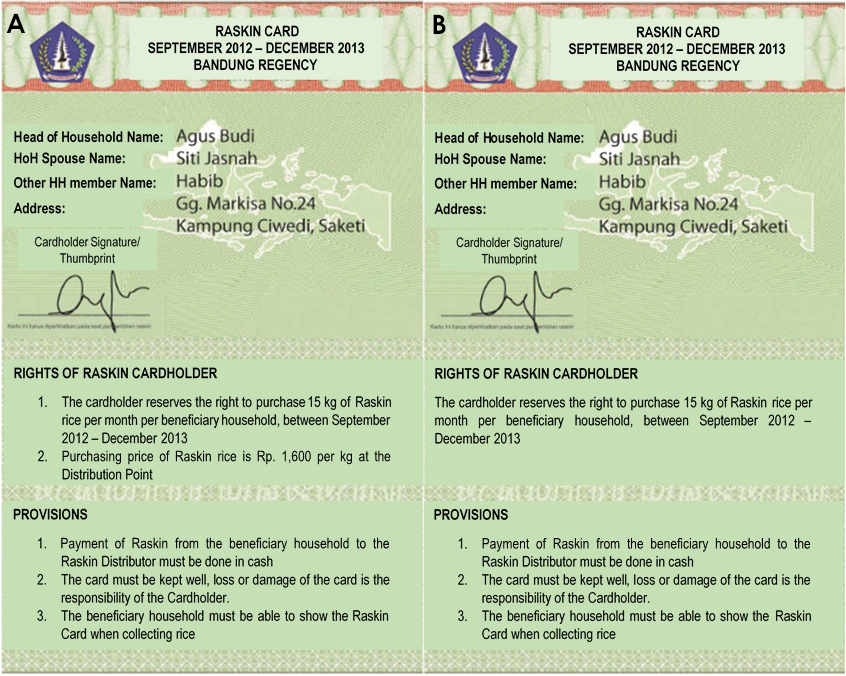
\includegraphics[width=1\linewidth]{./figures/indonesiafigure1} \caption{Sample Raskin cards. The names in these sample cards are fictitious and for demonstration purposes only. }\label{fig:indonesiafigure1}
\end{figure}

Note: the names in these sample cards are fictitious and for demonstration purposes only.

\hypertarget{using-administrative-data-to-monitor-an-experimental-treatment}{%
\subsection{Using Administrative Data to Monitor an Experimental Treatment}\label{using-administrative-data-to-monitor-an-experimental-treatment}}

The government of Indonesia (GoI) aims to convert its five principal social protection programs, known as \emph{Bantuan Sosial}, to electronic vouchers distribution by 2022. Collectively, these programs reach over 15 million of Indonesia's poorest households. According to a Presidential Decree issued in June 2016, the Raskin\index{Raskin} rice program was slated first to make the transition.

Beginning this process, the government of Indonesia transitioned Raskin from an in-kind transfer to e-vouchers. Under the new system, called BPNT\index{BPNT} (\emph{Bantuan Pangan Non-Tunai}/Non-Cash Food Assistance), beneficiary households are transferred electronic vouchers directly to an account in their name that they can access using a debit card, smart card, or mobile money platform. Recipient households can then theoretically redeem these e-vouchers at a network of agents (registered shops or vendors) for rice or eggs. These include both public-sector agents as well as private retailers who are recruited and equipped to accept BPNT e-vouchers by one of Indonesia's state-owned banks.

While the research team worked with the GoI on the overall evaluation\index{evaluation} of the reform (see \protect\hyperlink{building-questions-into-the-national-sample-survey-to-measure-outcomes}{Building Questions into the National Sample Survey to Measure Outcomes}, below), the researchers also aimed to understand whether the number of agents in the area affected the quality of the BPNT\index{BPNT} program (i.e., whether a more competitive market improves quality). The government had issued initial guidelines specifying (1) an agent to beneficiary ratio of at least 1:250 in each village and (2) a minimum of two agents per village. However, very few areas were meeting these requirements, and it was important to understand how much effort and how many resources the government should exert to increase compliance.

In 2016, working with the GoI, the research team identified 216 districts where the BPNT reform had already happened or was in progress. The team then randomized the districts into two experimental groups. In one group, the districts are asked to exert extra effort to try to meet the agent coverage requirements. In the second group, districts were told that one of the two coverage guidelines was no longer required. The banks tasked with recruiting private BPNT agents and district officials learned of each district's treatment status through the normal processes for sharing programs and policies with stakeholders: letters from the government, a series of explanatory meetings, and phone calls to reinforce the treatment.

\begin{figure}
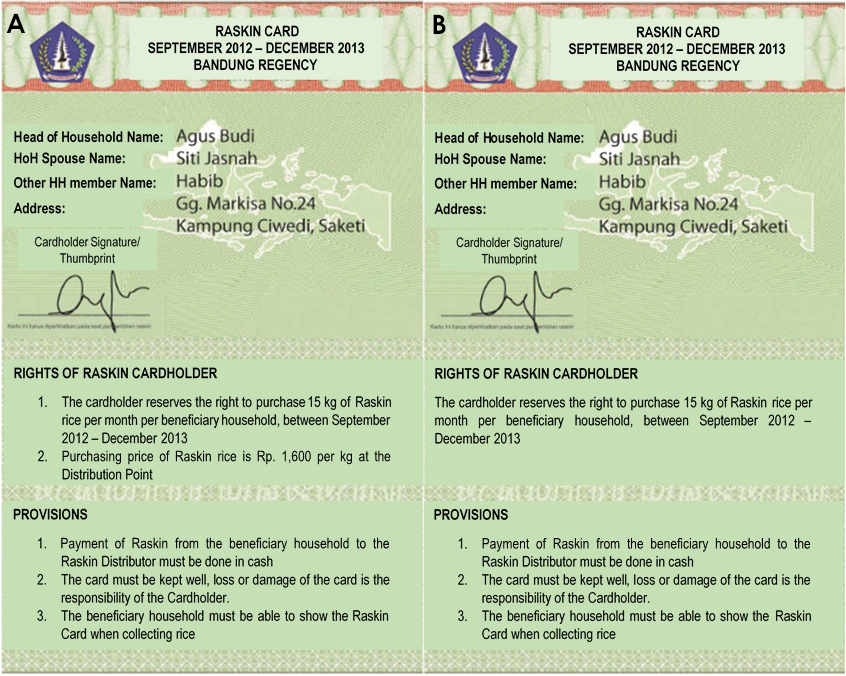
\includegraphics[width=1\linewidth]{./figures/indonesiafigure2} \caption{State-owned banks recruit private retailers to serve as BPNT agents and outfit them with equipment to process BPNT e-voucher transactions and some time to provide other basic banking services. These recruited agents then appear in bank administrative data.}\label{fig:indonesiafigure2}
\end{figure}

As part of the design, the researchers had to monitor the experiment and understand whether the number of BPNT agents actually changed as a result of treatment activities (e.g., letters, meetings), and whether villages met the GoI-issued requirements.

Given the spread of the districts across the nation, surveying villages across the 216 districts (and visiting each one multiple times to capture changes over time) would have been prohibitively expensive. Instead, the research team used administrative data to monitor the experiment.

The researchers obtained detailed administrative data from the banks tasked with the recruitment of BPNT agents, collected by Bank Indonesia (Indonesia's Central Bank) to learn how many agents existed within each village, with snapshots twice a year starting March 2018. This data on bank agents is provided by each of the government banks participating in the program as part of regular administrative data reporting on their agent recruitment activities.

In an example of the kind of troubleshooting often required when working with administrative data, once the research team ascertained that the data are available and could be used to monitor the intervention---and, more generally, the reform---the team discovered that the form and codes of cataloguing villages and districts were not consistent across banks, nor consistent with the government's official codes. This made it difficult to match data both across different data sets and across time. The research team provided support to the government and the banks to clean the data and work with the institutions to draft guidelines to make the data consistent across various data sets going forward. In this case, collaboration between the research team and the government resulted in improvements to the data collection process, facilitating further research and program implementation.

\hypertarget{using-administrative-data-to-measure-outcomes}{%
\section{Using Administrative Data to Measure Outcomes}\label{using-administrative-data-to-measure-outcomes}}

In most experimental program evaluation designs, one measures the \emph{actual outcomes} of both the control and treatment groups by conducting an endline survey. This can be costly. For example, a basic, two-hour endline survey across households for the Raskin\index{Raskin} card example costs about US\$60--\$70 per household surveyed, not including additional independent survey monitoring costs. The expense of these surveys can add up quickly when surveying a large sample or measuring program impact at various points in time (e.g., short-run versus long-run outcomes). The following two sections describe how two different forms of administrative data (program use data and national sample surveys) were used to measure program outcomes.

\hypertarget{utilizing-program-use-data-to-measure-outcomes}{%
\subsection{Utilizing Program Use Data to Measure Outcomes}\label{utilizing-program-use-data-to-measure-outcomes}}

In January 2014 the GoI introduced a national health insurance\index{health insurance} scheme, Jaminan Kesehatan Nasional (JKN), with the objective of achieving universal insurance coverage by 2019. JKN is a contributory system run by the Social Security Agency (BPJS Kesehatan). Non-poor informal workers are mandated to individually register for JKN and make monthly payments, but the mandate is hard to enforce. Unsurprisingly, BPJS Kesehatan has faced low take-up among this group. Those who do enroll tend to be those who have high levels of claims, so the revenues generated by premium payments do not cover the high cost.

A discussion began among researchers, TNP2K, BPJS Kesehatan, and Bappenas in 2014 to understand how to address this take-up issue. An experiment was designed to test whether temporary price subsidies could boost enrollment among healthier individuals, driving down the government's cost per individual enrolled.\footnote{Additional treatments were also designed to understand how both non-monetary sign-up costs and informational barriers affected take-up (see \citet{banerjee2019} for more details on the experimental treatments and results).}

The experiment and data collection process in the two sample cities (Medan and Bandung) ran roughly as follows. Since there was no list of non-poor, informal workers who were not enrolled in JKN, researchers first went door-to-door to find individuals. Through this method, the research team identified about 6,600 target households for the sample. The researchers then conducted a short baseline survey that included the NIK (national ID number) of each household member, so that the sample could be matched to the BPJS administrative data. After the survey, households were individually randomized into different arms of the experiment through the survey app, and the survey enumerator administered the corresponding subsidy treatment (if any).

To understand the effect of the treatments on take-up, enrollment (i.e., selection), and ultimately the per person cost of insurance to the government, the researchers matched the NIK numbers of sample respondents to the BPJS administrative data on enrollments, monthly premium payments, and claims over the subsequent 32 months to answer three questions (for both the treatment and control groups):

\begin{enumerate}
\def\labelenumi{\arabic{enumi}.}
\tightlist
\item
  Did the household enroll?
\item
  Did the household stay enrolled (i.e., did they continue to make their monthly premium payments)?
\item
  Did the household utilize the insurance? More specifically, did they visit a health care provider? What was the visit for? How much did the government need to reimburse the provider (i.e., the value of the health claim)?
\end{enumerate}

The administrative data had several advantages over conducting a conventional household survey. First, it was much cheaper, since the data used were collected as part of the program administration, instead of just for the experiment. Second, recall bias was not a concern with the administrative data. Imagine the researchers had run an endline survey two and a half years after the treatment instead of using the administrative data. People could have easily forgotten the exact month when they visited the doctor and for what reason. To mitigate recall bias in a survey context, one would conduct frequent endline surveys to capture timely data, but this strategy can easily double or triple survey costs. Instead, with the administrative data, the research team had dated information for the 32-month follow-up period that was not subject to recall bias. Third, an endline survey may have been subject to differential response bias: households who received the treatment might feel indebted or grateful to the researchers and thus more inclined to respond positively to questions about the insurance. The administrative data obviated this concern, as it recorded actual, observed insurance outcomes for everyone.

\protect\hyperlink{indonesia-appendixa}{Appendix A} describes the close collaboration between the research team and the GoI that ultimately ensured the safe use of Indonesia's national health insurance\index{health insurance} data in this research project. In the end, the systems put in place to facilitate data use paid off in terms of policy impact. The research collaboration provided key insights to the Indonesian government on their insurance pricing systems---Bappenas credited the collaborative study on the national health insurance system when determining insurance premium pricing in 2016.

\hypertarget{building-questions-into-the-national-sample-survey-to-measure-outcomes}{%
\subsection{Building Questions into the National Sample Survey to Measure Outcomes}\label{building-questions-into-the-national-sample-survey-to-measure-outcomes}}

As discussed in \protect\hyperlink{using-administrative-data-to-monitor-an-experimental-treatment}{Using Administrative Data to Monitor an Experimental Treatment}, the government of Indonesia has transitioned Raskin\index{Raskin} from an in-kind transfer of rice to e-vouchers redeemable for rice or eggs. This system was introduced in 44 of the largest cities in 2017 as a pilot, with a larger rollout in 54 cities and selected districts in 2018, and a national rollout in 2019.

The GoI asked for assistance to assess the impact of the reform on the quality of services that beneficiaries receive, which was to be studied around the 2018 phase-in of the reform. Given the budget allocation for 2018 to serve about 8.3 million beneficiaries with BPNT\index{BPNT}, the government needed to choose about 40--45 districts from 105 districts that were ready to receive the program during the 2018 roll-out, with the remaining districts to be treated under the budget allocations for 2019. Thus, the researchers randomized 42 districts to receive BPNT in 2018, with the rest treated in mid-2019.

A key question was how to survey citizens to evaluate the reform. The experiment spanned 105 districts across the country, making conventional household survey methods infeasible as discussed in \protect\hyperlink{using-administrative-data-to-monitor-an-experimental-treatment}{Using Administrative Data to Monitor an Experimental Treatment}, above. With the GoI, the research team identified an alternative. Since 1963--64, the Statistics Bureau of the Government of Indonesia (BPS) has conducted a biennial national sample survey\index{national sample survey} called the National Socioeconomic Survey (SUSENAS). It is administered to over 250,000 households and collects data on health, education, fertility, consumption and expenditures, and housing, among others. SUSENAS data are used for various purposes including planning, monitoring, and evaluating government programs. The researchers thus developed an idea to add questions to the SUSENAS to evaluate the BPNT\index{BPNT} reform. The SUSENAS is particularly well-suited for this use, as it covers all districts and is representative at the district level (the researchers' unit of randomization).

\protect\hyperlink{indonesia-appendixb}{Appendix B} describes the process of adding questions to the national sample survey\index{national sample survey} through careful collaboration with many stakeholders. A challenge was ensuring that the timelines matched between the program implementation and the survey. The national sample survey has a set schedule determined by BPS, while the schedule for the transition of districts to BPNT (the treatment in this experiment) was decided by other ministries. Coordination was necessary to ensure that the treatment groups were transitioned to BPNT sufficiently before the surveys were fielded and that the control groups were treated afterwards.

The national sample survey represents a hybrid between administrative data and experiment-specific survey data. The survey is in the form of a conventional household survey but is administered by the government in order to inform its policies, regardless of the specific research projects described here. More generally, note that using national sample survey data of this sort has benefits and limitations. Benefits include large geographic scope and representative samples. The survey constitutes a panel of districts, and so control variables at the district level from previous years can be included in regression models to gain additional statistical power. In terms of limitations, as one can imagine from the process above, adding questions to a national survey may not provide all the variables that would be desired in a two-hour, evaluation-specific endline survey. In fact, the new Block XVI on Social Protection was only one page long, so questions needed to be designed very carefully.

\hypertarget{studying-the-collection-of-administrative-data-itself}{%
\section{Studying the Collection of Administrative Data Itself}\label{studying-the-collection-of-administrative-data-itself}}

As described in Using Administrative Data To Implement An Experimental Treatment, a number of programs in Indonesia use the UDB---a unified database of the households that are eligible for government programs. A series of studies conducted by members of this research team explored a variety of ways how to do this best (in particular \citet{alatas2012}, \citet{alatas2016}).

\hypertarget{administrative-data-collection-for-program-targeting}{%
\subsection{Administrative Data Collection for Program Targeting}\label{administrative-data-collection-for-program-targeting}}

Governments are often worried about whether social assistance reaches the poorest households. In 2005, the government of Indonesia announced cuts to fuel subsidies, which were to be offset by increased transfers to the poor and near-poor. Program targeting\index{Program targeting} emerged as an important policy priority, as the government sought to ensure that these transfers reached their intended recipients. In 2011, to further improve the targeting of social protection programs\index{social protection programs}, Indonesia set out to establish a national targeting system.\footnote{Indonesia has historically used a blend of methods. For example, BLT, a cash transfer program launched in 2005, relied mostly on community assessment, self-assessment. and pre-existing lists to collect data and has relied mostly on PMT (proxy-means test) scores and community input to select beneficiaries from the resulting pool. The village head nominated poor individuals, and theoretically, this nomination data was combined with pre-existing lists of family planning data. However, in practice, frequently only the village head nominations were used. In 2008, data collection methods for the cash transfer program were supposedly modified to use consultative community meetings to update lists, identifying households that had moved, died, or were no longer poor. However, in practice, these meetings were generally restricted to village officials, rather than the broader community, and households were only removed for death or relocation, not for no longer being poor.} This national targeting system, the Unified Data Base (UDB\index{UDB}), is essentially a unified registry of actual and potential beneficiaries, which aims to provide high-quality data for all programs to access, facilitate complementarities between programs, reduce costs by avoiding duplicated targeting efforts across programs, and mitigate fraud, corruption, and the unintended duplication of benefits. While the potential advantages of such a system are large, switching targeting methods introduces the risk that some households could be systematically excluded from social assistance. The technical and administrative challenges of such a multi-program effort are extensive, and the risk of information manipulation may increase with the scale of the effort.

To mitigate these risks, careful decisions on data collection and selection were needed, and a number of options for collecting this administrative data were considered. In particular, there was debate as to whether to conduct a survey sweep with hard data collection enabling the use of a proxy-means test\index{proxy-means test} (see Using Administrative Data to Implement an Experimental Treatment and Using Administrative Data as a Research Treatment to Improve Data Collection), community-based targeting, or some combination of both. In collaboration with the government, researchers from J-PAL and the World Bank conducted a randomized control trial to test these targeting methods against each other \citep{alatas2012}.

The results of the experiment informed the creation of the Data Collection for Social Protection Programs (PPLS11) registry, which was finalized in December 2011, covering the 25 million poor and vulnerable households constituting Indonesia's bottom 40 percent. It was subsequently endorsed by a cabinet-level committee, which instructed all central agencies to use it as the basis of their beneficiary lists. The registry has since been used for the national health fee waiver program (Jamkesmas) that aims to cover the poorest 76 million individuals and a conditional cash transfer program that now covers 10 million households, as well as for targeting unconditional cash transfers to qualifying households during further fuel subsidies reductions (see Using Administrative Data to Implement an Experimental Treatment). The establishment and widespread use of this registry significantly reduced the exclusion of poor households from government assistance, marking a critical milestone in Indonesia's development of an integrated social safety net. Furthermore, since the adoption of PPLS11, Indonesia has continued to improve its administrative data systems, and thus the social protections that rely on those systems, through empirical research that relies on both experimental and administrative data. One follow-up study focused on the potential of using self-selection to help determine inclusion in the proxy-means test screening process \citep{alatas2016}.

\hypertarget{using-administrative-data-as-a-research-treatment-to-improve-data-collection}{%
\subsection{Using Administrative Data as a Research Treatment to Improve Data Collection}\label{using-administrative-data-as-a-research-treatment-to-improve-data-collection}}

In 2014, the government of Indonesia set about updating the UDB, which forms the basis of eligibility of social protection programs\index{social protection programs}. The UDB contains data from a semi-census where Census Bureau enumerators collect information from households on socioeconomic characteristics and assets. These data are then fed into the proxy-means test formula used to identify poor households and target them for social programs.

One important question in both the economics literature and policy space is whether these data collection processes used in program targeting have distortionary effects. In high-income countries, where means testing is done based on employment and income status, the question often revolves around whether targeting leads to individuals working less for fear of becoming disqualified from benefits programs. Since targeting is based on assets in low-income countries (as income and employment are hard to verify), the question becomes whether households would choose not to invest in assets (or hide assets) for similar reasons. This could have real implications on household well-being, for example, if the asset is a better water source that can affect health or a productive asset (like a cow) that can affect household consumption.

Working in partnership with the government of Indonesia, the researchers built a randomized controlled trial directly into the 2015 UDB data collection---which collected data on 25 million households, generating data on 92 million individuals nationally---to ascertain whether adding additional asset questions to the UDB data collection would incentivize households to reduce asset acquisition.

Specifically, the researchers randomized questions about two additional assets onto the UDB\index{UDB} questionnaire. The randomization was done at the province-level, since that is the level at which the surveys are printed and the enumerators are trained. To ensure that everyone received the same number of survey questions, each province was randomized into one of two options: in half the provinces, households received (1) either a question on flat-screen television ownership or a question on the number of rooms in their house and (2) either a question on how many active cell-phone SIM card numbers the household had or whether they had a modern toilet installed. Importantly, TVs and cell phones can be hidden from enumerators far more easily than rooms and toilets. Thus, the researchers could test whether being exposed to a particular question affected citizens reported and actual asset ownership.

Inserting different variables for randomization required the approval from the BPS deputy in charge of social statistics. For the data collection, BPS had to train approximately 100,000 enumerators, which spanned central, provincial, and district level trainings. Having different versions of the questionnaire within the same data collection was a new exercise for BPS and so was the idea of randomization. Despite the challenges that the new data collection posed, the researchers were able to convince the BPS deputy to implement the randomization because of a long history of engagement and collaboration between BPS and TNP2K, along with a presentation to BPS leaders on the rationale and future benefits of the study. Additionally, the BPS deputy also benefited from the opportunity to check the quality of SUSENAS data. In order to understand the treatment impacts on actual cell phone ownership, the researchers obtained administrative data on yearly SIM card subscribers from all major Indonesian telecommunications companies through the Ministry of Communications and Informatics (KeMenKomInfo). Following formal written requests from TNP2K and presentations regarding the study's objective to KeMenKomInfo officials, they finally agreed to release the data strictly for the purpose of the study. The study found that households randomized to receive the TV question were less likely to report TV ownership, but actual TV sales were unaffected, suggesting that households may have responded by hiding the asset, not changing their consumption.

\hypertarget{concluding-remarks-5}{%
\section{Concluding Remarks}\label{concluding-remarks-5}}

The experiences discussed here suggest that administrative data has a number of roles to play in conducting research on social protection policies. The projects described use administrative data as an outcome variable, allowing the scalable use of high-quality data. Even beyond that, the researchers used administrative data to implement treatments and in addition studied how to improve administrative data collection itself.

Several key lessons emerge. Given that governments own most administrative data sets, it is important to determine research questions and priorities together with the government so that the study is policy relevant. It is imperative to keep in mind that there are often multiple stakeholders; researchers must make sure that everyone understands the study goals, the exact data that are needed, the manner data will be used, and the responsibilities on both sides. Given the sensitivity of some data, having strong data storage protocols that meet IRB standards is important.

It is of course worth noting that administrative-data based experiments do not work in all cases and have some costs. For example, in some instances, an intervention would need to be designed, randomized, and implemented at a much larger scale (e.g., district level rather than village level) in order to match the available data. In other cases, the types of questions needed may not be available in existing data sets (for example, self-reported health status is not available in health insurance claim data). Notwithstanding, the projects and resulting policy actions described here would not have been feasible without leveraging administrative data through collaborations with many stakeholders---a crucial resource for researchers and policymakers seeking to generate and use experimental evidence for social good.

\hypertarget{about-the-authors-10}{%
\section*{About the Authors}\label{about-the-authors-10}}
\addcontentsline{toc}{section}{About the Authors}

\href{https://www.hks.harvard.edu/faculty/rema-hanna}{Rema Hanna} and \href{https://economics.mit.edu/faculty/bolken}{Benjamin Olken} are the scientific directors of J-PAL SEA and \href{https://economics.mit.edu/faculty/banerjee}{Abhijit Banerjee} and Benjamin Olken are both directors of J-PAL. \href{https://www.povertyactionlab.org/person/widyasari}{Putu Poppy Widyasari} is a research manager at J-PAL SEA, and \href{https://www.povertyactionlab.org/person/amalia}{Farah Amalia} is a senior training associate at J-PAL SEA. \href{https://www.smeru.or.id/en/content/sudarno-sumarto}{Sudarno Sumarto} is senior research fellow at the SMERU Research Institute and a policy adviser at TNP2K. Vivi Alatas was lead economist at the World Bank during the work discussed here.

\hypertarget{acknowledgements-4}{%
\section*{Acknowledgements}\label{acknowledgements-4}}
\addcontentsline{toc}{section}{Acknowledgements}

We thank the many J-PAL SEA staff members who contributed to the projects discussed here, in particular Lina Marliani for many years of outstanding leadership of J-PAL Southeast Asia and Alexa Weiss and Jenna Juwono for comments and input on the draft. We thank our many partners in the Government of Indonesia, in particular Bambang Widianto, Suahasil Nazara, Pungky Sumadi, Vivi Yulaswati, Andi ZA Dulung, Tubagus A Choesni, Fachmi Idris, Mundiharno, Tono Rustiano, Wynandin Imawan, Rahmi Artati, Maliki, Elan Satriawan, Gantjang Amanullah, M.O Royani, Nurul Farijati, Herbin, Dwi Martiningsih, Andi Afdal, Citra Jaya, Thoman Pardosi, Sri Kusumastuti Rahayu, and Fiona Howell for outstanding cooperation. Funding for the research described here came from the Australian Government Department of Foreign Affairs and Trade, the World Bank--Royal Netherland Embassy Trust Fund, 3ie, KOICA, and the Harvard Ash Center, along with in-kind support from the Government of Indonesia. We thank Survey Meter and Mitra Samya for outstanding data collection, project implementation, and fieldwork. Alatas was a Senior Economist at the World Bank during the work discussed here, and Sumarto works as a Policy Advisor to the Indonesian Government through TNP2K. The views expressed here are those of the authors alone and do not necessarily represent any of the institutions or individuals acknowledged here.

\begin{invisible}
This is a workaround for citations in footnotes, please ignore.
@newhouse1993 @behrman1999 @gertler2004
\end{invisible}

\putbib

\FloatBarrier\newpage

\hypertarget{indonesia-appendix}{%
\section*{Appendix}\label{indonesia-appendix}}
\addcontentsline{toc}{section}{Appendix}

\hypertarget{indonesia-appendixa}{%
\subsection*{Appendix A}\label{indonesia-appendixa}}
\addcontentsline{toc}{subsection}{Appendix A}

\textbf{Collaborating to work with Indonesia's health insurance records}

First, researchers and government partners discussed the research questions, study priorities, and treatments. This ensured that the study questions were useful for policy. This is an important first step for any evaluation collaboration to be successful, regardless of whether administrative data are used.

Second, the relationship was formalized through two agreements that clearly outlined the research design and plan, the data that would be shared with the researchers, and the responsibilities of each actor. The initial agreement was a memorandum of agreement between BPJS Kesehatan (who owned the data), Bappenas (who was facilitating the research from the policy side), and J-PAL SEA (who represented the researchers). This agreement included the study design, broad data to be shared, and the study protocols. The other agreement was a separate cooperation agreement between BPJS Kesehatan and J-PAL SEA that spelt out each entity's roles and responsibilities in detail. Both agreements required a series of official meetings that occurred over the course of six months.

Next, the official data request was submitted to BPJS Kesehatan. This included the exact variables to be shared, the frequency of data sharing, the de-identification process, and the data security protocols in place. The administrative data from the national insurance program are sensitive. It contains not only insurance status but also health records. Therefore, it was very important that both the government and researchers followed these data protection principles: (1) to ensure that the data were used for the stated purposes only, (2) that all parties were in agreement on those purposes, and (3) that strict data security protocols were followed. At this point, the research team was working closely with BPJS Kesehatan to understand the structure of the data, how it could be extracted, which departments within BPJS were responsible for the different component data sets, and so forth.

After an official letter was issued to grant data access, the research team maintained a close relationship with the BPJS team to continue to discuss the data use and ask questions about the data sets themselves. In addition, periodic updates on the results were presented to the BPJS team so that they could learn from the experiment as it was happening.

\hypertarget{indonesia-appendixb}{%
\subsection*{Appendix B}\label{indonesia-appendixb}}
\addcontentsline{toc}{subsection}{Appendix B}

\textbf{Collaborating to embed questions in Indonesia's official national sample survey}

Adding questions to a national sample survey seemed like a straightforward idea, especially since the survey was being conducted anyway and the evaluation itself was commissioned by the government. But as with most things in life, things are never so simple.

It is important to keep in mind that the government comprises many different actors and each has a stake in the data, as they have their own policy information needs. Thus, the first challenge was to identify the stakeholders in this data set and generate buy-in. One clear stakeholder is BPS (the census bureau), who is in charge of conducting the sample survey and ultimately decides what to include.

However, many different ministries use the SUSENAS data, submit their own sets of questions to BPS, and have input and feedback on the overall survey. Moreover, given that BPS has a fixed budget to field the survey, there are constraints on the survey length. If questions are added, it likely means that others are removed. Therefore, the research team had to ensure buy-in from other ministries that would be interested in the BPNT\index{BPNT} reform to increase the probability that the submitted questions were included.

Therefore, in addition to numerous meetings and discussions with BPS to explain the importance of adding the questions and maintaining them over several rounds, the research team also conducted a series of meetings with other stakeholders, including Bappenas, TNP2K, the Ministry of Social Affairs (MoSA), and the Coordinating Ministry for Human Development and Cultural Affairs (PMK).

A second challenge was to follow the right timeline for stakeholder engagement and attend the right meetings where decisions were made. For example, the research team found that in order to include new questions in the regular SUSENAS data collection in March, discussions with related ministries and institutions need to start at the latest in July or August of the previous year, before survey preparation begins in September. Inter-ministerial coordination usually occurs in October when the ministries propose their own questions for SUSENAS. This coordination workshop is crucial, since this is where the decisions to keep or drop questions are made. The research team therefore obtained permission to attend the workshop.

The first draft of the questionnaire from the inter-ministerial meeting is then workshopped internally by BPS and circulated with several representatives from each relevant institution in early November. During this process, modifications are still highly possible. Since the activity is usually not public (i.e., only between BPS and each ministry or institution separately), regular follow-up with BPS is necessary to understand the current stage of the process. By following up with government partners, such as TNP2K and Bappenas, the research team was able to access several drafts of the questionnaires and provide inputs as necessary. Ultimately, the additional questions proposed by the research team were approved by BPS and included in the socioeconomic survey, specifically in Block XVI on Social Protection, a new section in the SUSENAS used to track the reform.
